\documentclass[11pt,letterpaper]{article}
\usepackage[T1]{fontenc}
\usepackage{amsmath}
\usepackage{newtxtext}
\usepackage{newtxmath}
\usepackage[letterpaper,left=1.65cm,right=1.65cm,top=1.52cm,bottom=1.65cm]{geometry}
\usepackage{microtype}
\usepackage{booktabs,tabularx,array}
\usepackage{tikz}
\usepackage{titlesec}
\usepackage{caption}
\usepackage[hidelinks]{hyperref}
\hypersetup{pdftitle={Shopping and Budget Advisor},pdfauthor={Hechuan ZHANG, Bolin CHEN, Jieming CHEN}}
\linespread{0.93}
\setlength{\parindent}{0pt}
\setlength{\parskip}{1.2pt}
\setlength{\tabcolsep}{4pt}
\setlength{\emergencystretch}{1em}
\titleformat{\section}{\fontsize{12}{13}\selectfont\bfseries}{\thesection}{0.5em}{}
\titlespacing*{\section}{0pt}{5pt}{3pt}
\DeclareCaptionFont{compact}{\fontsize{9}{10.2}\selectfont}
\captionsetup{font=compact,labelfont=bf,skip=3pt,hypcap=false}
\definecolor{app}{HTML}{EFF4FF}
\definecolor{know}{HTML}{EDF8F3}
\definecolor{train}{HTML}{F0F2FC}
\definecolor{infer}{HTML}{FFF6E9}
\definecolor{eval}{HTML}{F5F0FC}
\definecolor{infra}{HTML}{EEF7FB}
\definecolor{appink}{HTML}{2855A5}
\definecolor{knowink}{HTML}{21785B}
\definecolor{trainink}{HTML}{5555A2}
\definecolor{inferink}{HTML}{986516}
\definecolor{evalink}{HTML}{74539C}
\definecolor{infraink}{HTML}{28738D}
\newcommand{\archrow}[6]{%
  \fill[fill=#2,rounded corners=3pt] (0,#1) rectangle (518,{#1+27});
  \fill[fill=#2ink,rounded corners=1pt] (0,{#1+4}) rectangle (2,{#1+23});
  \node[anchor=west,text=#2ink,text width=87pt,inner sep=0pt,font=\fontsize{9}{10.2}\selectfont\bfseries] at (8,{#1+13.5}) {#3};
  \node[archcard] at (99,{#1+13.5}) {#4};
  \node[archcard] at (239,{#1+13.5}) {#5};
  \node[archcard] at (379,{#1+13.5}) {#6};
}
\begin{document}
\begin{center}
{\fontsize{17}{19}\selectfont\bfseries Shopping and Budget Advisor}\\[2pt]
{\fontsize{10.5}{12}\selectfont CSIT6000T Course Project Proposal}\\[1pt]
{\fontsize{10.5}{12}\selectfont Hechuan ZHANG, Bolin CHEN, Jieming CHEN}
\end{center}
\vspace{-8pt}

\section{Motivation and task}
A low listing price can become a poor choice once delivery charges, missing accessories, or unsuitable specifications are considered. Reviews may refer to different versions, repeat claims, or disagree about important attributes. For a basket, substitutions also change whether the purchase meets the budget. Buyers must check evidence across sources and decide which tradeoffs fit their needs.

We propose a shopping and budget advisor for any user group and product category. Individuals, households, and teams need recommendations that reflect intended use and available funds. Users will describe essential requirements and possible compromises. The advisor will compare alternatives, explain tradeoffs with source evidence, and revise plans as priorities change, leaving the purchase decision with the user.

We will handle one request at a time and return ranked products or baskets with itemized costs, links, tradeoffs, and remaining funds. Users may set a purchase cap or supply a periodic budget, spending, and a reserve. When both limits are given, available funds are the smaller of the cap and the balance after spending and reserves. Missing essential specifications or costs trigger clarification.

\section{Proposed system}
Six layers (Figure~\ref{fig:architecture}) extend the repository's TACC deployment and inference client with shopping, knowledge, and evaluation capabilities. Training and new quantization depend on available resources.
\begin{center}
\vspace{-3pt}
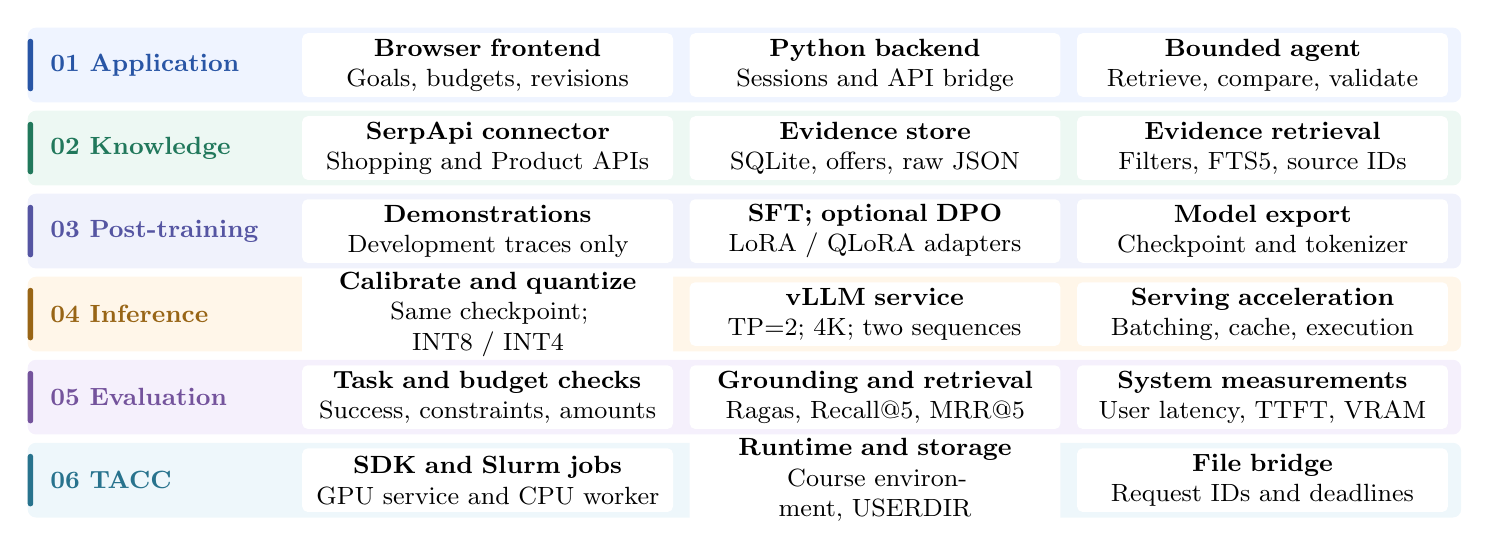
\begin{tikzpicture}[x=1pt,y=1pt,archcard/.style={anchor=west,draw=none,fill=white,rounded corners=2pt,text width=126pt,minimum height=23pt,inner xsep=4pt,inner ysep=1pt,align=center,font=\fontsize{8.6}{11}\selectfont}]
\archrow{150}{app}{01 Application}{\textbf{Browser frontend}\\Goals, budgets, revisions}{\textbf{Python backend}\\Sessions and API bridge}{\textbf{Bounded agent}\\Retrieve, compare, validate}
\archrow{120}{know}{02 Knowledge}{\textbf{SerpApi connector}\\Shopping and Product APIs}{\textbf{Evidence store}\\SQLite, offers, raw JSON}{\textbf{Evidence retrieval}\\Filters, FTS5, source IDs}
\archrow{90}{train}{03 Post-training}{\textbf{Demonstrations}\\Development traces only}{\textbf{SFT; optional DPO}\\LoRA / QLoRA adapters}{\textbf{Model export}\\Checkpoint and tokenizer}
\archrow{60}{infer}{04 Inference}{\textbf{Calibrate and quantize}\\Same checkpoint; INT8 / INT4}{\textbf{vLLM service}\\TP=2; 4K; two sequences}{\textbf{Serving acceleration}\\Batching, cache, execution}
\archrow{30}{eval}{05 Evaluation}{\textbf{Task and budget checks}\\Success, constraints, amounts}{\textbf{Grounding and retrieval}\\Ragas, Recall@5, MRR@5}{\textbf{System measurements}\\User latency, TTFT, VRAM}
\archrow{0}{infra}{06 TACC}{\textbf{SDK and Slurm jobs}\\GPU service and CPU worker}{\textbf{Runtime and storage}\\Course environment, USERDIR}{\textbf{File bridge}\\Request IDs and deadlines}
\end{tikzpicture}
\captionof{figure}{Planned architecture. SerpApi feeds the knowledge base; budget tools validate plans; post-training targets agent behavior.}
\label{fig:architecture}
\vspace{-5pt}
\end{center}

\textbf{01 Agent Application Layer.} A browser will collect goals and budgets and support progress, sources, and revisions. The backend will maintain sessions; a bounded agent will clarify, retrieve, compare, and validate. Schema-checked Python tools will check requirements, quantities, known taxes/shipping, and exact totals.

\textbf{02 Knowledge Layer.} Backend SerpApi Shopping and Product calls will acquire listings and available offers, specifications, and reviews [1]. Sanitized JSON and persistent SQLite records will preserve variants, sources, currency, and timestamps. Deduplication will retain conflicts; filters and FTS5 will retrieve cited evidence. Live refreshes are API-budgeted; evaluation uses immutable snapshots.

\textbf{03 Post-Training Layer.} Development demonstrations will teach clarification, evidence selection, tool calls, and recovery. SFT with LoRA/QLoRA requires a trainable checkpoint; DPO is optional. Held-out cases and the unseen category are excluded from training and calibration. Exports retain tokenizer and model configuration.

\textbf{04 Quantization and Inference.} Supported INT8/INT4 variants will share a checkpoint and generation settings. The initial vLLM service uses tensor parallelism of two, 4K context, and at most two sequences. Context selection, batching, caching, and execution modes will be compared for quality, latency, and total GPU memory.

\textbf{05 Evaluation Layer.} A harness will replay frozen requests and log model/snapshot IDs, prompts, seeds, observations, tokens, timing, and errors. Rules and human review will distinguish retrieval, tool-use, arithmetic, and serving failures.

\textbf{06 TACC Infrastructure Layer.} Tcloud/Slurm will run a GPU service on two observed 24\,GiB GPUs and a separate CPU worker. An SDK file bridge keeps model calls inside TACC; public API calls and credentials stay on the backend. USERDIR persistence, deadlines, and job states support one-hour allocations.

\newpage
\section{Evaluation plan}
\textbf{Representative tasks and quality.} We will prepare 10 development and 40 held-out cases across five categories; eight cases test a fifth category added through schemas and data after freezing the agent, prompts, and tools. Cases cover products, baskets, unit-price differences, budget boundaries, substitutions, revisions, and incomplete evidence. Independent enumeration of the frozen catalog will establish feasibility and exact costs. Task success rate (TSR) requires a feasible, correctly priced plan, a correct catalog-limited no-plan report, or a necessary clarification; unnecessary abstention is failure. We target zero budget violations and arithmetic errors and report two reviewers' preference-fit scores (1--5). A shared rubric will score specification fit, justified tradeoffs, and completeness. Unknown shipping or taxes must remain explicit; an unsupported estimate cannot establish affordability. Revision cases will check that unchanged requirements persist.

\textbf{Knowledge base and retrieval.} With about 100 products and 300 review excerpts where available, we will audit field coverage, duplicates, source agreement, and price age. Reviewers will label relevant evidence for Recall@5 and MRR@5. Ragas Context Precision/Recall, Faithfulness, and Factual Correctness will supplement citation support/coverage checks [2]. Faithfulness measures consistency with supplied evidence, not whether prices remain current. Retrieval comparisons will share structured candidates, prices, the model, and budget tools; missing/stale facts will be distinguished from retrieval errors. Product variants will receive stable IDs; near-duplicate reviews will stay within the same data split. References will be labeled before viewing system outputs, with disagreements resolved against archived evidence.

\textbf{Baselines and efficiency.} Table~\ref{tab:baselines} specifies controlled baselines and ablations. Base/SFT comparisons share a base model; precision comparisons share a trained checkpoint. We will vary sequential/two-way analysis, filtered/unfiltered context, and serving settings one factor at a time. Each held-out case will run three times per core configuration, interleaved on the same endpoint, with case-paired uncertainty. The target is 20\% lower median latency or 30\% fewer input tokens versus the sequential, unfiltered agent, with at most a five-percentage-point success loss. Timeouts, malformed outputs, stale offers, and missing fees will be injected, with at least one failure trace analyzed. Development will proceed from SDK transport and data ingestion to retrieval, deterministic budget tools, and the complete agent. Baseline evaluation precedes adapter training and quantization; each stage must pass the same frozen task checks.

\vspace{3pt}
\begingroup
\fontsize{9.3}{10.7}\selectfont
\renewcommand{\arraystretch}{1.12}
\begin{tabularx}{\linewidth}{@{}lXrrrr@{}}
\toprule
\textbf{Method} & \textbf{Configuration} & \textbf{TSR \% $\uparrow$} & \textbf{Faith. $\uparrow$} & \textbf{BVR \% $\downarrow$} & \textbf{p95 s $\downarrow$}\\
\midrule
B0 Single call & No extra text; no budget tool & n/m & n/m & n/m & n/m\\
B1 Keyword RAG & FTS5; single call; no budget tool & n/m & n/m & n/m & n/m\\
B2 Structured RAG & Filtered FTS5; single call; no budget tool & n/m & n/m & n/m & n/m\\
\textbf{B3 Full advisor} & B2 + bounded loop + budget tool & n/m & n/m & n/m & n/m\\
\midrule
A1 Without loop & B3; one-pass plan with the same tools & n/m & n/m & n/m & n/m\\
A2 Without validator & B3; budget tool disabled & n/m & n/m & n/m & n/m\\
\bottomrule
\end{tabularx}
\endgroup
\captionof{table}{Planned baseline and ablation results; n/m = not measured. Faithfulness is on a 0--1 scale; p95 is full-request latency. Budget violation rate (BVR) uses delivered plans as its denominator. All methods share structured candidates and prices. A1 isolates the loop; A2 isolates the validator.}
\label{tab:baselines}

\vspace{4pt}
\begingroup
\fontsize{9.5}{11}\selectfont
\renewcommand{\arraystretch}{1.08}
\begin{tabularx}{\linewidth}{@{}p{0.17\linewidth}X@{}}
\toprule
\textbf{Pipeline stage} & \textbf{Measures and measurement boundary}\\
\midrule
Acquisition / KB & Required-field coverage, source agreement, duplicates, price age; API calls, refresh/cache state, errors, and acquisition latency.\\
Retrieval & Recall@5 and MRR@5 from evidence IDs; Context Precision/Recall from ranked evidence and reference facts [2].\\
Answer / agent & Faithfulness, Factual Correctness, citation coverage, preference fit; schema validity and Tool Call Accuracy [2,3].\\
Budget / task & TSR, BVR, hard-constraint violations, and exact amount error from independent feasibility and arithmetic checks.\\
Model serving & TTFT, TPOT, ITL, request/output-token throughput, SLO goodput, and peak total GPU memory [4].\\
Whole request & User p50/p95 latency, completion/failure rate, tokens, API/LLM calls, and cost per successful task; trace queue/bridge/tool spans.\\
\bottomrule
\end{tabularx}
\endgroup
\captionof{table}{Full-pipeline measurement. TTFT = time to first token; TPOT = time per output token; ITL = inter-token latency; SLO = service level objective. The current blocking client needs streaming instrumentation to measure token timing.}

\textbf{Reporting controls.} Freeze snapshots for quality comparisons and report live acquisition separately. Warm up serving and separate cold starts/cache states. Model TTFT excludes earlier acquisition and bridge waits. Include failures, API retries, and unsuccessful tasks in cost accounting; freeze SLO thresholds on development cases. Ragas judges will be versioned and checked against human labels; deterministic budget checks remain authoritative. We will report paired bootstrap intervals over cases, preserving repeated runs within each case. BVR is undefined when no plans are delivered. Throughput gains will be interpreted alongside successful tasks per unit time. Reports will archive model and runtime configurations, case definitions, snapshot manifests, evaluation scripts, and representative traces for reproducibility.

\vspace{2pt}
{\fontsize{9}{10.2}\selectfont
\textbf{References.}
[1] \href{https://serpapi.com/google-shopping-api}{SerpApi Shopping} / \href{https://serpapi.com/google-product-api}{Product APIs}.
[2] \href{https://docs.ragas.io/en/stable/concepts/metrics/available_metrics/}{Ragas RAG metrics}.
[3] \href{https://docs.ragas.io/en/stable/concepts/metrics/available_metrics/agents/}{Ragas tool metrics}.
[4] \href{https://docs.vllm.ai/en/latest/benchmarking/cli/}{vLLM benchmarks}.}
\end{document}
